\section{Resultats}
\captionsetup[figure]{labelsep=space}
\subsection{Descripció de les dades}

\begin{figure}[h!]
\centering
\begin{minipage}{0.45\linewidth}
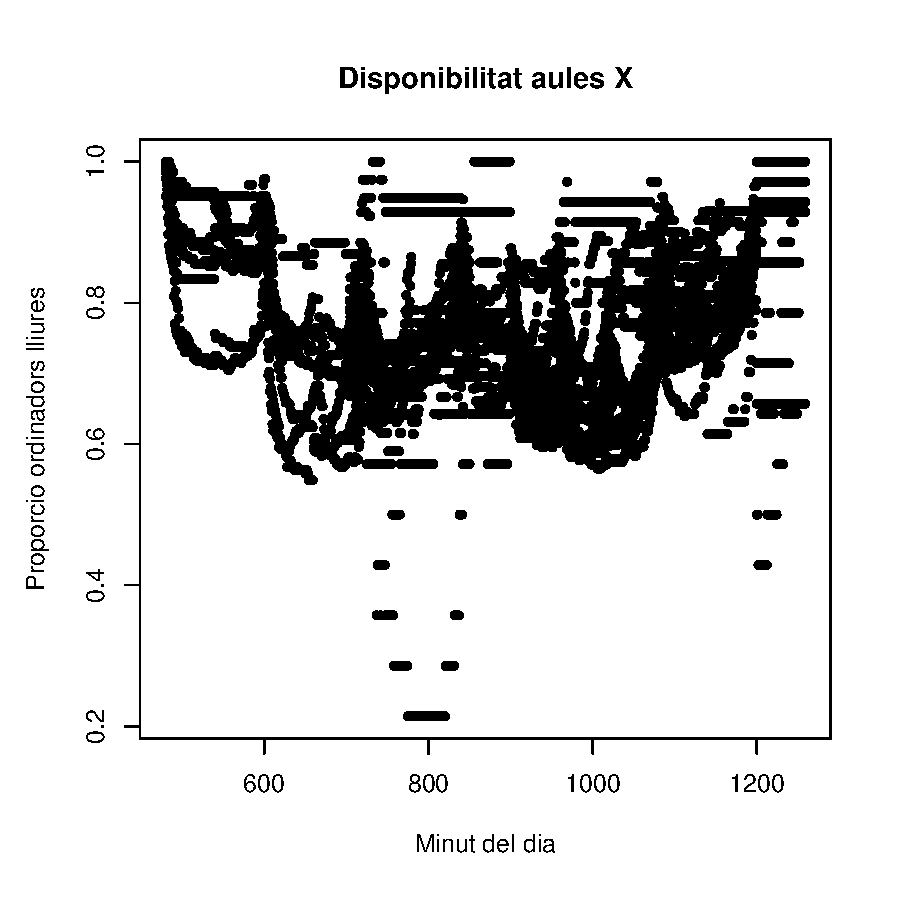
\includegraphics[width=1\linewidth]{./images/dades_X.eps}
\end{minipage}
\hfill
\begin{minipage}{0.45\linewidth}
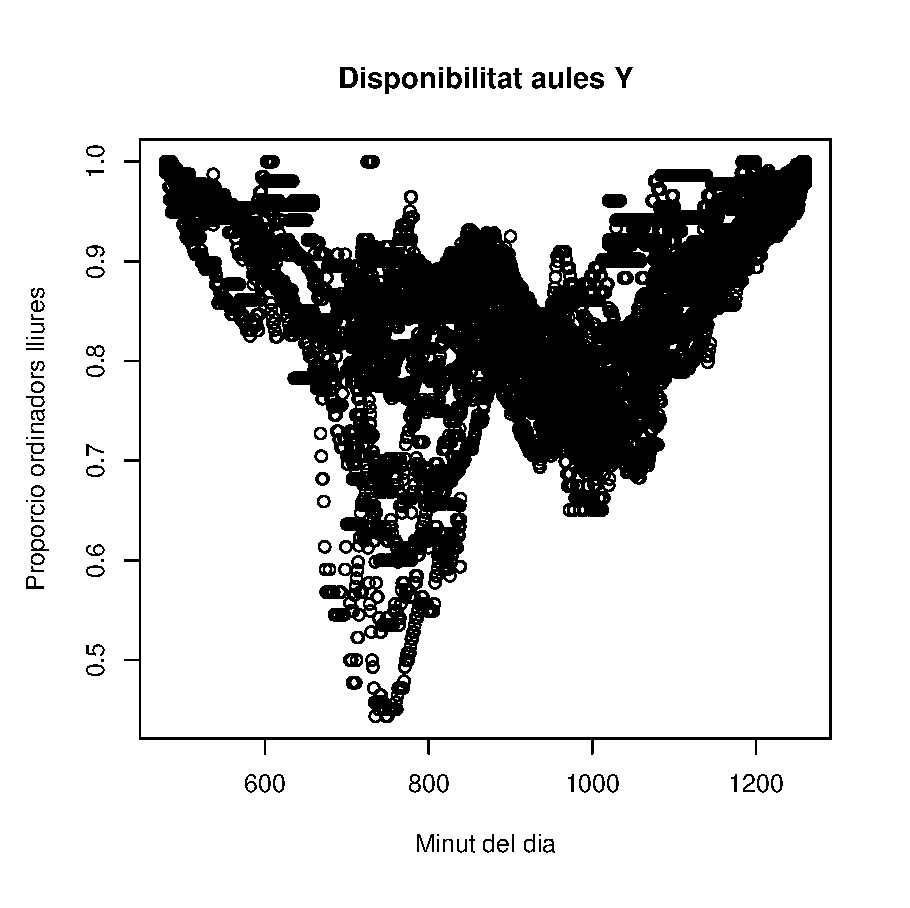
\includegraphics[width=1\linewidth]{./images/dades_Y.eps}
\end{minipage}
\end{figure}

Els dos primers gràfics són els reculls de dades per les aules amb classe i les aules sense classe. Cada punt és la proporció d'ordinadors lliures en una hora en concret.

En les premisses hem suposat que l'estadístic $\hat{z}$ es podia aproximar a una normal. A les figures \ref{fig:densY} i \ref{fig:densX} podem veure que les variables \emph{X} i \emph{Y} s'assemblen lleugerament al gràfic d'una distribució normal. La figura \ref{fig:qqplot} mostra la desviació de $X-Y$ respecte a una normal. Observant aquesta i la figura \ref{fig:histograma} es pot veure que la diferència entre \emph{X} i \emph{Y} (que és proporcional a $\hat{z}$) segueix una normal amb una petita anormalitat en els valors més petits.

Les dades completes es poden trobar en un full de càlcul seguint el següent enllaç:\\
\url{https://docs.google.com/spreadsheets/d/1elGJjdaar26Jyu9gmvHlC1y-p9IX4dDBx0xu2t6Q0hw/pubhtml}

\begin{figure}
\centering
\begin{minipage}{0.45\linewidth}
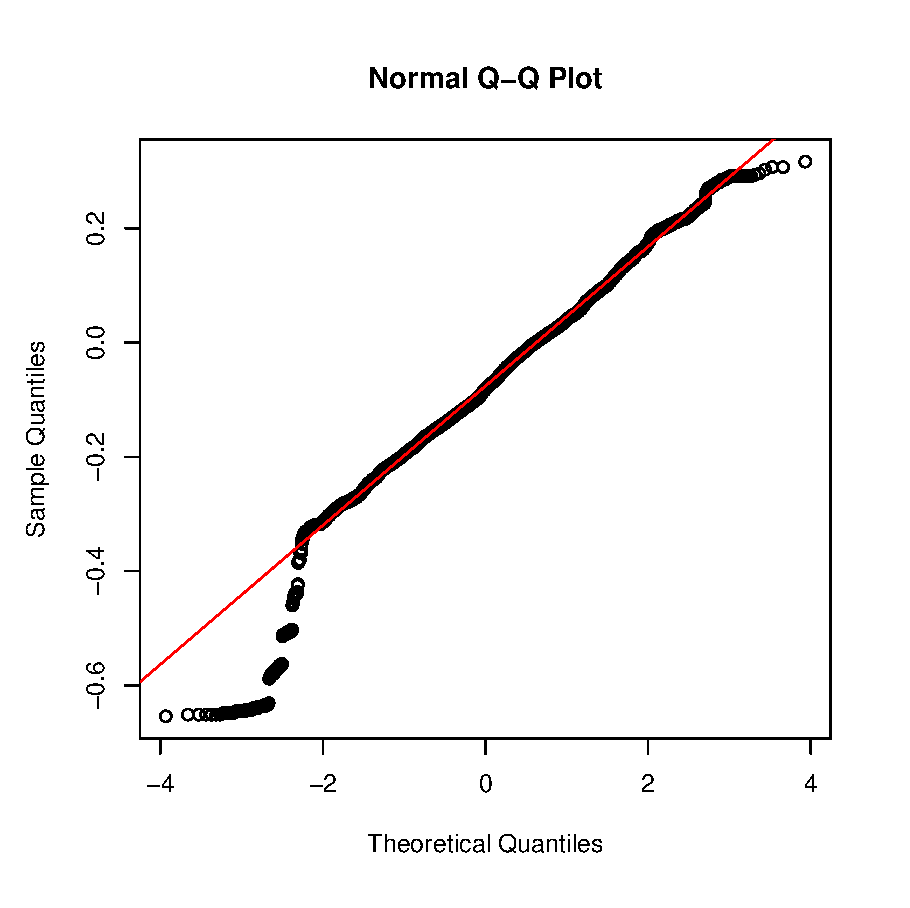
\includegraphics[width=1\linewidth]{images/qqplot}
\caption{}
\label{fig:qqplot}
\end{minipage}
\hfill
\begin{minipage}{0.45\linewidth}
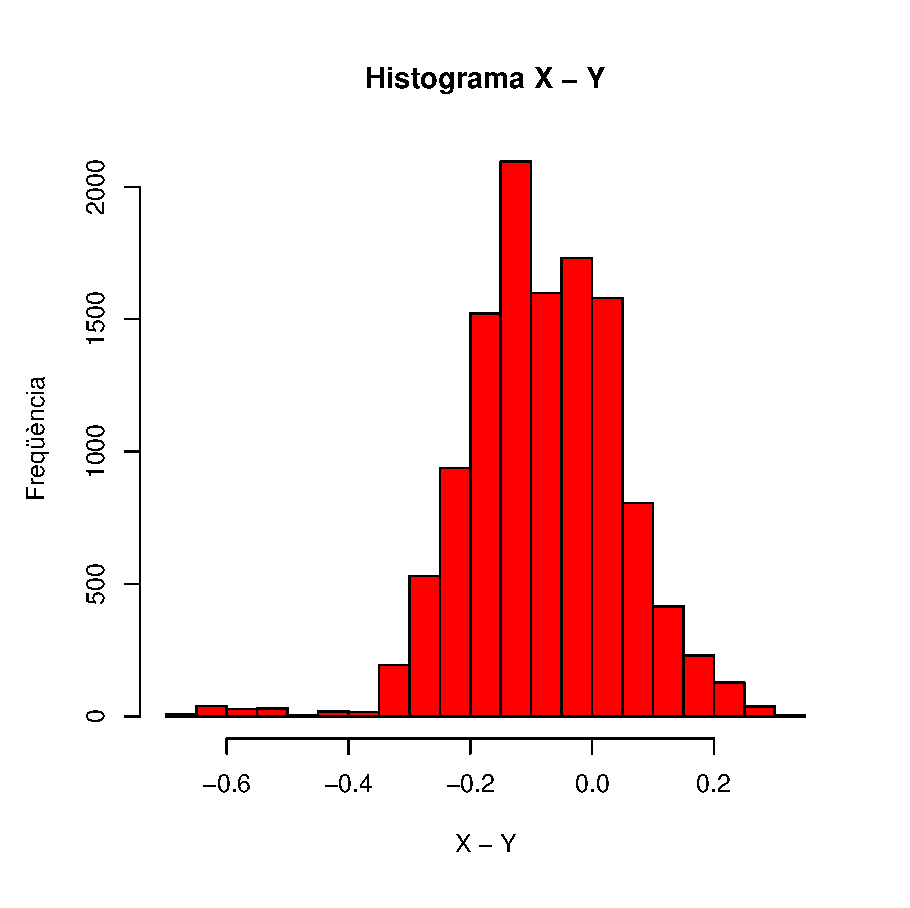
\includegraphics[width=1\linewidth]{images/histograma}
\caption{}
\label{fig:histograma}
\end{minipage}
\end{figure}

\subsection{Comparació de la disponibilitat}


\begin{figure}[h!]
\begin{minipage}{0.5\linewidth}
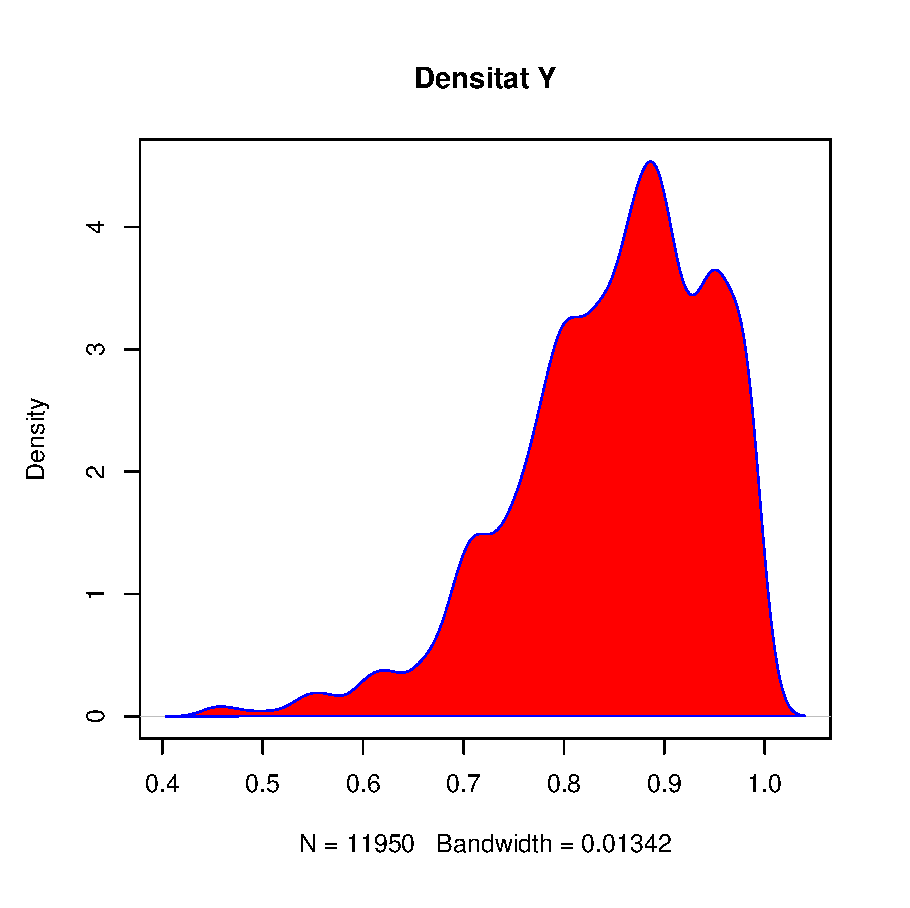
\includegraphics[width=1\linewidth]{./images/no_DENS.eps}
\caption{}
\label{fig:densY}
\end{minipage}
\hfill
\begin{minipage}{0.5\linewidth}
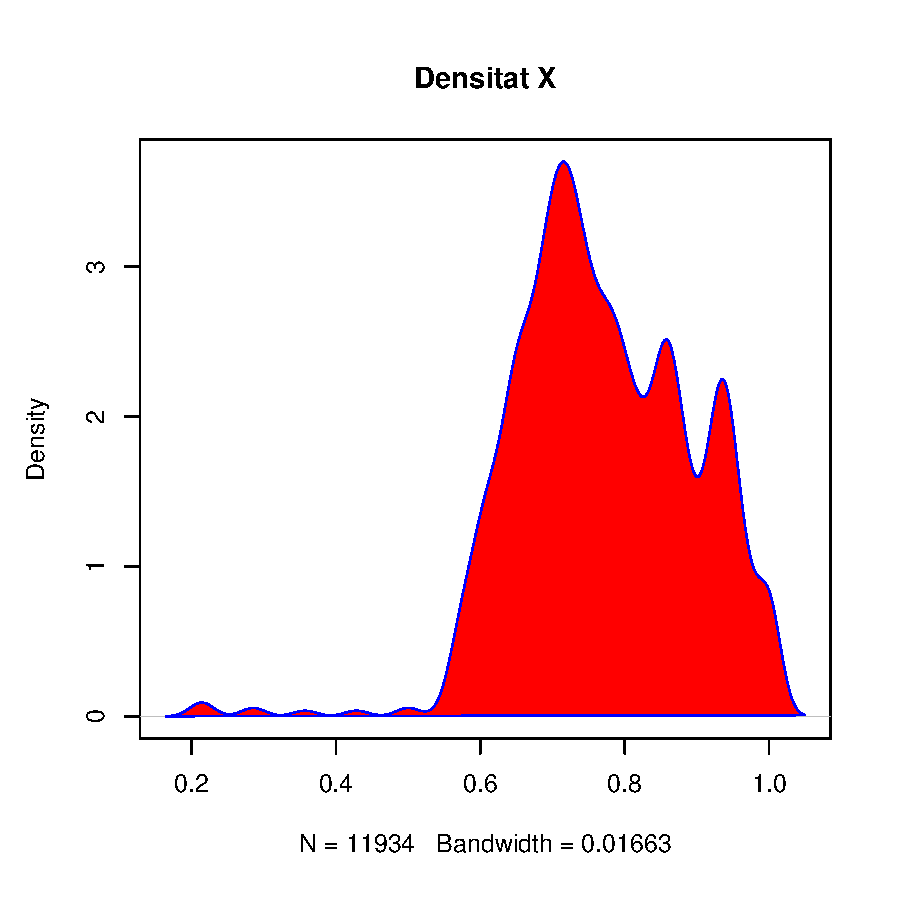
\includegraphics[width=1\linewidth]{./images/si_DENS.eps}
\caption{}
\label{fig:densX}
\end{minipage}
\end{figure}
Analitzant les dades obtingudes hem arribat als següents valors:
$$\bar{x} = 0.77083, s^2_x = 0.01459139, n_x = 11934$$
$$\bar{y} = 0.8503347, s^2_y = 0.009507904, n_y = 11950$$
I per tant:
$$\hat{z} = -55.96263$$


El valor de $\hat{z}$ és extremament petit. De fet, calculant el p-valor amb \emph{R} per aquesta $\hat{z}$ el resultat és 0. Per tant, queda clar que s'ha de rebutjar la hipòtesi nul·la. És més, degut a que $\hat{z}$ ha resultat ser negativa, podem afirmar que $\mu_Y > \mu_X$.